\documentclass{beamer}
%[aspectratio=169]   \usepackage[czech]{babel}
\usepackage{apo-lecture}
\usepackage{pdfpages}
\usepackage{pdfcomment}
\usepackage{listings}
\usepackage{array,multirow}

\subtitle{Lekce 08. Výukový kit MZ\_APO (Xilinx Zynq MicroZed APO)}
\author{Pavel Píša \phantom{xxxxxxxxx} Petr Štěpán \\ \small\texttt{pisa@fel.cvut.cz}\phantom{xxxx}\small\texttt{stepan@fel.cvut.cz}}
\begin{document}

\maketitle

\section{MZ\_APO -- Xilinx Zynq MicroZed výukový kit pro B35APO}

\begin{frame}
\frametitle{Cíl dnešní přednášky}

\begin{itemize}
 \item Seznámení s koponemtami/kontrukcí výukového kitu
 \item Komunikace a základní práce s kitem
 \item Princip a přístup na displej z tekutých krystalů (LCD)
 \item Barevné modely pro vykreslování
 \item Výstup písma
 \item Využití HW pro reálné aplikace
\end{itemize}
\end{frame}

\begin{frame}
\frametitle{Výukový kit MZ\_APO -- smontovaný}

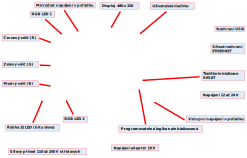
\includegraphics[width=0.98\textwidth]{mz_apo-kit-with-cover-labels.pdf}

\end{frame}

\begin{frame}
\frametitle{Výukový kit MZ\_APO -- základová deska}

\includegraphics[width=1.0\textwidth]{mz_apo-baseboard-top-labels.pdf}

\end{frame}

\begin{frame}
\frametitle{Modul MicroZed -- pohled shora}

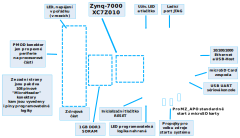
\includegraphics[width=1.0\textwidth]{microzed-board-top-labels.pdf}

\end{frame}

\begin{frame}
\frametitle{Modul MicroZed -- pohled zespodu}

MicroZed Evaluation Kit -- ADSAES-Z7MB-7Z010-G (případně AES-Z7MB-7Z010-SOM-G/REV-H cena 214\,USD)
\par
SoM -- počítač na modulu (System on Module)
\par
Čip Xilinx/AMD XC7Z010, cena okolo 90\,USD (2023)
\par
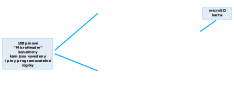
\includegraphics[width=0.90\textwidth]{microzed-board-bottom-labels.pdf}
\par
108-pinové konektory umožňují využít a propojit modul s vlastním návrhem. I přes tyto piny je možné modul napájet,
přítup k PS periferiím i pinům programovatelné logiky PL (FPGA).

\end{frame}

\begin{frame}
\frametitle{Modul MicroZed -- katalogový list}

\begin{itemize}
 \item Čip FPGA – Zynq™-7000 AP SoC (XC7Z010-CLG400-1)
 \begin{itemize}
  \item CPU: Dual ARM® Cortex™-A9 MPCore™ @ 866 MHz
  \item rychlá vnitřní statická paměť 256 kB
  \item 4400 řezů (slice) - každý řez je malý konfigurovatelný logický obvod.
    Dokáže vytvořit až 8 klopných obvodů a 4 logické funkce se 6-ti vstupy.
    Uživatel je může libovolně konfigurovat a vzájemně propojovat.
 \end{itemize}
 \item Externí dynamická paměť – 1 GB DDR3
 \item Komunikace – 10/100/1000 Ethernet
 \item MicroSD karta 4 GB. V desce APO obsahuje zavaděč systému Linux pro síť Ethernet.
 \item USB Host 2.0 a USB-UART
 \item Quad-SPI Flash 128 Mb pro inicializaci při zapnutí.
 \item V APO se nepoužívá.
\end{itemize}
\end{frame}

\begin{frame}
\frametitle{Zynq™-7000 AP -- pouzdro FBGA}

\begin{columns}
\begin{column}{0.5\textwidth}
  \begin{center}
    FBGA = Fine-Pitch Ball Grid Array
    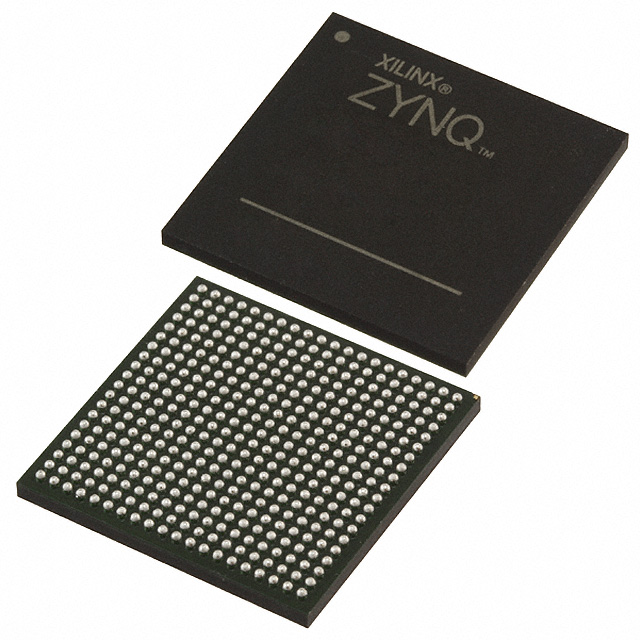
\includegraphics[width=1.0\textwidth]{fig/zynq-fbga-package.jpg}
  \end{center}
  \vfil
\end{column}
\begin{column}{0.5\textwidth}
  \begin{center}
    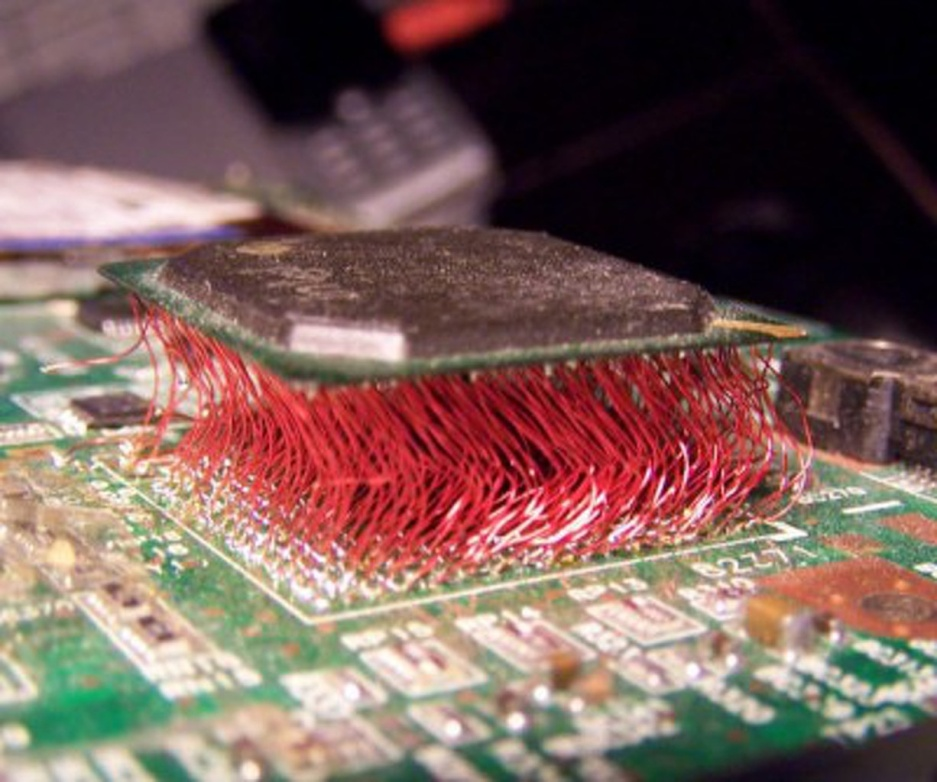
\includegraphics[width=0.55\textwidth]{fig/bga-soldering-clumsy.jpg}
    \newline
    Kuriózní pájení
    \newline
    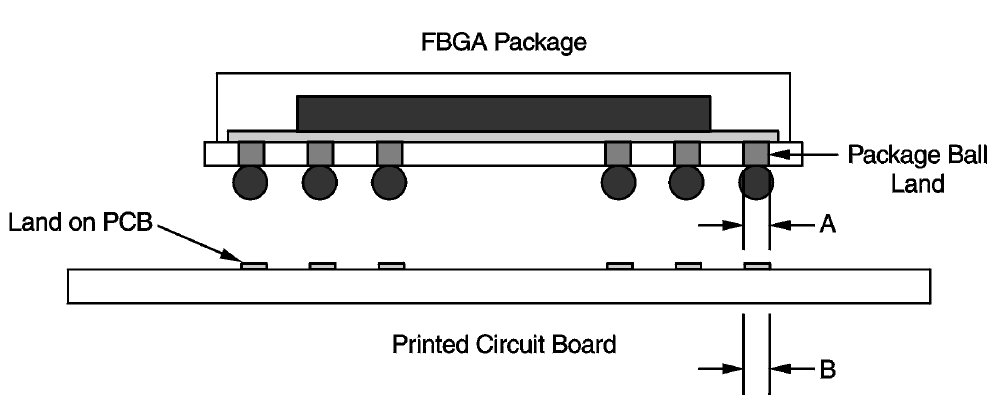
\includegraphics[width=0.8\textwidth]{fig/bga-dimensions-diagram.png}
    \newline
    Korektní pájení
    \newline
    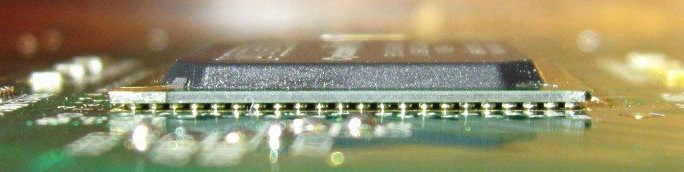
\includegraphics[width=0.8\textwidth]{fig/bga-soldering-proper.jpg}
  \end{center}
\end{column}
\end{columns}

\end{frame}


\begin{frame}
\frametitle{MZ\_APO -- návrh v programu Vivado}
  \begin{center}
    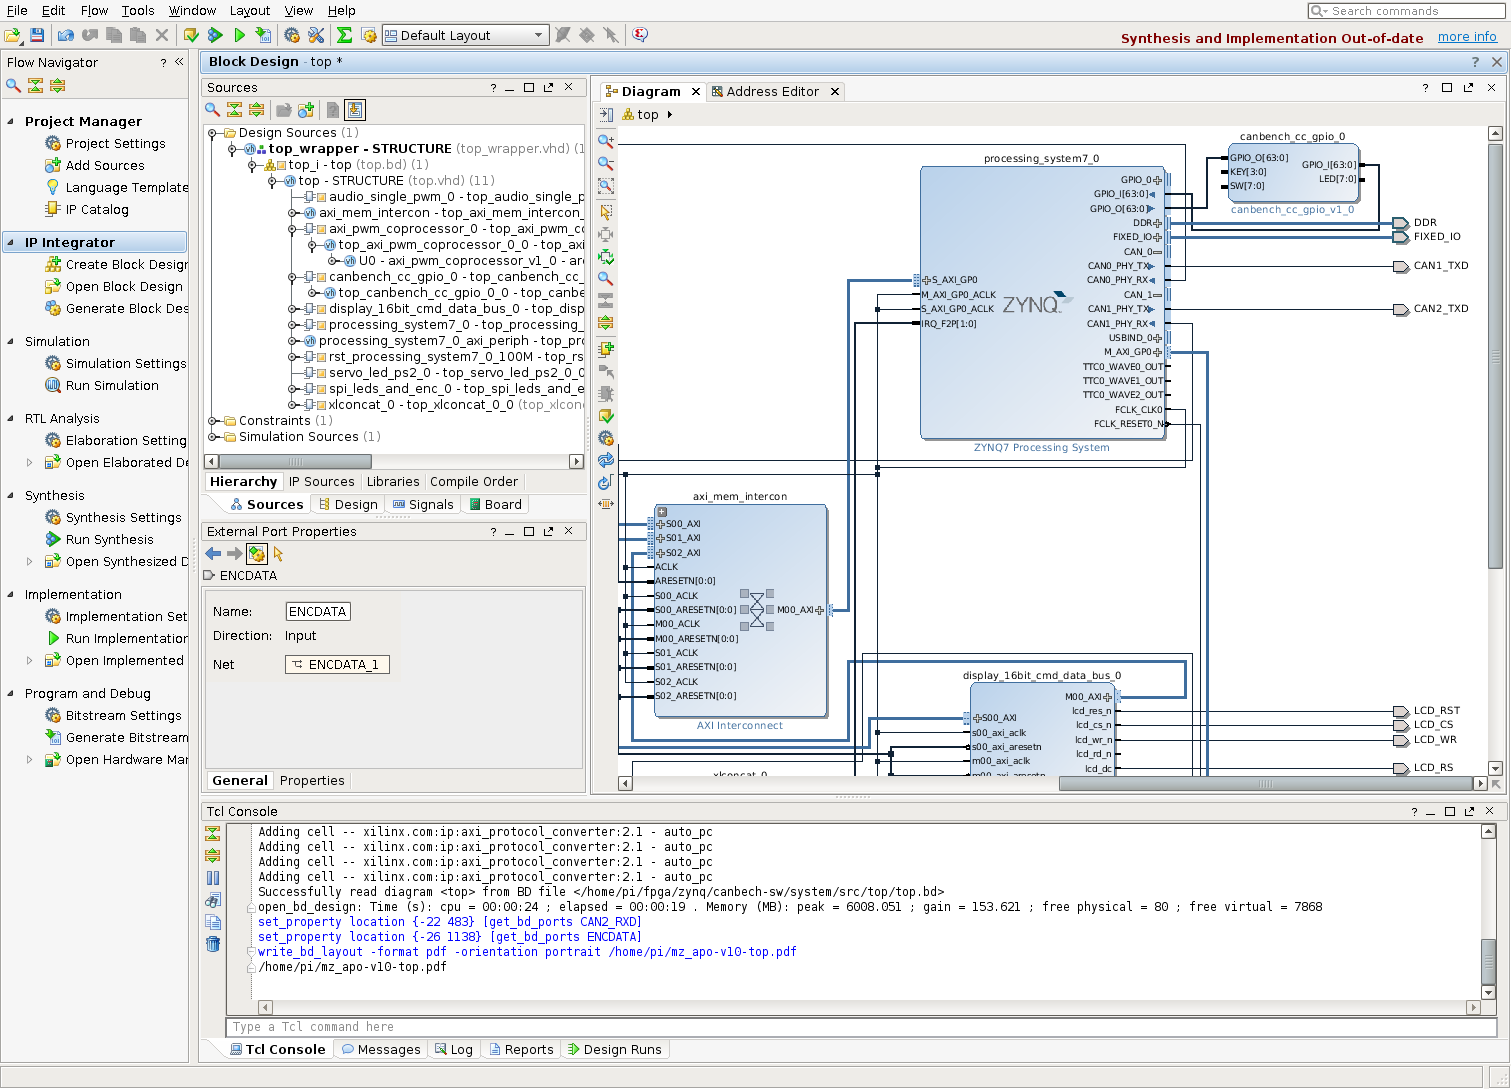
\includegraphics[width=0.85\textwidth]{fig/mz_apo-vivado-screenshot.png}
  \end{center}
\end{frame}


\begin{frame}
\frametitle{MZ\_APO -- logický návrh sběrnic}

\includegraphics[width=1.0\textwidth]{mz_apo-vivado-design.pdf}

\end{frame}



\begin{frame}
\frametitle{MZ\_APO -- indikátory LED a otočné voliče}

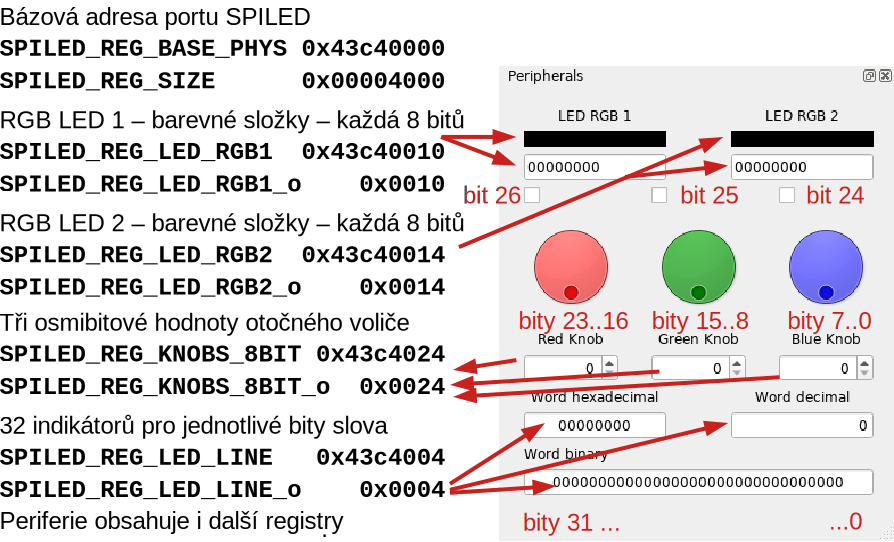
\includegraphics[width=1.0\textwidth]{mz_apo-spiled-and-knobs-cz.pdf}

\end{frame}



\begin{frame}
\frametitle{Zápis na displej na kitu MZ\_APO}

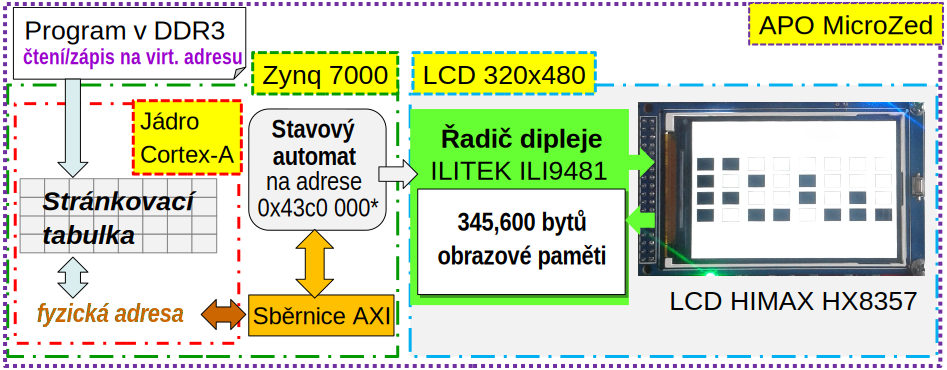
\includegraphics[width=0.9\textwidth]{mz_apo-lcd-access-cz.pdf}

\end{frame}



\end{document}

